\subsection{Motivation}
\begin{frame}
	\frametitle{Background}
	\begin{itemize}
		\item France 
		\begin{itemize}
			\item Preparation for a transition from \glspl{LWR} to \glspl{SFR} \cite{cne2_reports_2015}
			\item Additional \gls{LWR} construction to supply Plutonium for \gls{SFR} transition
		\end{itemize}
		\item Most EU nations do not have a repository for \gls{UNF}
	\end{itemize}
\end{frame}

\begin{frame}
	\frametitle{Summary}
	By taking \gls{UNF} from other EU nations, France can transition into a fully \gls{SFR} fleet (66 GWe capacity)
	without additional construction of \glspl{LWR}.
	\begin{itemize}
		\item Transition to 110 \gls{ASTRID}-type \glspl{SFR} (Capacity 66 GWe)
		\item Collaborative approach benefits both sides
	\end{itemize}
\end{frame}

\begin{frame}
	\frametitle{Literature Review}
	Past research is mostly on:
	\begin{itemize}
		\item French transition to \glspl{SFR} after additional construction of \glspl{EPR} 	
		\cite{carre_overview_2009, martin_symbiotic_2017, freynet_multiobjective_2016}
		\item partitioning and transmutation in a regional (European) context \cite{fazio_study_2013}
	\end{itemize}

	There is little research on managing \gls{UNF} in a cooperative manner in
	advanced fuel cycles.
\end{frame}

\subsection{Method and Specfications}

\begin{frame}
	\frametitle{Cyclus}
	\Cyclus is the next generation agent-based nuclear \cite{huff_fundamental_2016}
	fuel cycle simulator.
	\begin{minipage}[b]{.45\linewidth}
	\begin{itemize}
		\item Flexibility to users and developers through a dynamic resource exchange solver
		\item user-developed agent framework
		\item low barrier to entry for new users and developers
		\item expanding ecosystem
	\end{itemize}
	\end{minipage}
	\hspace{.5cm}
	\begin{minipage}[b]{.45\linewidth}
	\begin{figure}
		\begin{center}
			
\includegraphics[width=\textwidth]{./images/cyclus.png}
		\end{center}
		% does this need a caption?
	\end{figure}
	\end{minipage}

\end{frame}


\begin{frame}
	\frametitle{Method}
	\Cyclus simulation of \gls{EU} nations (1970 - 2160) with 
	French Transition into an \gls{SFR} fleet from 2040.

\begin{figure}[htbp!]
        \begin{center}
                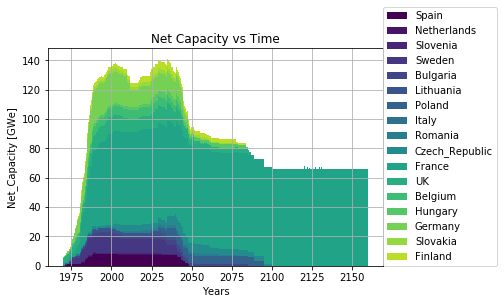
\includegraphics[width=.8\textwidth]{./images/onesim/power_plot.png}
        \end{center}
        \caption{Total Deployment Scheme of \gls{EU} nations}
        \label{fig:eu_dep}

\end{figure}

\end{frame}

\subsection{Future Projections}

\begin{frame}
	\frametitle{Future Deployment of Reactors in \gls{EU}}
	The power reactors listed in the table are used in the simulation
	to predict \gls{EU} \gls{UNF} inventory in 2050. 
	\begin{table}[h]
	\centering
	\caption {Power Reactors under construction and planned \cite{world_nuclear_association_nuclear_2017}}
	\label{tab:eu_deployment}
	\scalebox{0.70}{
	\begin{tabular}{ccccc}
		\hline
		\textbf{Exp. Operational} & \textbf{Country} & \textbf{Reactor} & \textbf{Type} & \textbf{Gross MWe}\\
		\hline
		2018 & Slovakia  & Mochovce 3 & PWR & 471 \\
		2018 & Slovakia & Mochovce 4 & PWR & 471 \\
		2018 & France & Flamanville 3 & PWR & 1600 \\
		2018 & Finland & Olkilouto 3 & PWR & 1720 \\		
		2019 & Romania & Cernavoda 3 & PHWR & 720 \\
		2020 & Romania & Cernavoda 4 & PHWR & 720 \\
		2024 & Finland & Hanhikivi & VVER1200 & 1200 \\
		2024 & Hungary & Paks 5 & VVER1200 & 1200 \\
		2025 & Hungary & Paks 6 & VVER1200 & 1200 \\
		2025 & Bulgaria & Kozloduy 7 & AP1000? & 950 \\
		2026 & UK & Hinkley Point C1 & EPR & 1670 \\
		2027 & UK & Hinkley Point C2 & EPR & 1670 \\
		2029 & Poland & Choczewo & N/A & 3000 \\
		2035 & Poland & N/A & N/A & 3000 \\
		2035 & Czech Rep & Dukovany 5 & N/A & 1200 \\
		2035 & Czech Rep & Temelin 3 & AP1000 & 1200 \\
		2040 & Czech Rep & Temelin 4 & AP1000 & 1200 \\
		\hline
	\end{tabular}
	}
\end{table}
\end{frame}


\begin{frame}
	\frametitle{Simulated European Deployment}
	
\begin{table}[h]
	\centering
	\begin{adjustbox}{max totalsize={1.1\textwidth}{.8\textheight}, center}
				\begin{tabularx}{\textwidth}{lmb}
					\hline 
					
					\textbf{Nation} & \textbf{Growth Trajectory} & \textbf{Specific Plan }\\
					\hline
					UK & Aggressive Growth & {\small  13 units (17,900 MWe) by 2030.}\\
					\hline
					Poland & Aggressive Growth &  {\small Additional 6,000 MWe by 2035.}\\
					\hline
					Hungary & Aggressive Growth &  {\small Additional 2,400 MWe by 2025.} \\ 
					\hline
					Finland & Modest Growth &  {\small Additional 2,920 MWe by 2024.}\\
					\hline
					Slovakia & Modest Growth & {\small Additional 942 MWe by 2025.}\\
					\hline
					Bulgaria & Modest Growth &  {\small Additional 1,000 MWe by 2035.} \\
					\hline
					Romania & Modest Growth &  {\small Additional 1,440 MWe by 2020.} \\
					\hline
					Czech Rep. & Modest Growth & {\small  Additional 2,400 MWe by 2035.}\\
					\hline
					France & Modest Reduction & {\small No expansion or early shutdown.}\\
					\hline
					Slovenia & Modest Reduction & {\small No expansion or early shutdown.}\\
					\hline
					Netherlands & Modest Reduction & {\small No expansion or early shutdown.}\\
					\hline
					Lithuania & Modest Reduction & {\small No expansion or early shutdown.}\\
					\hline 
					Spain & Modest Reduction &  {\small No expansion or early shutdown.} \\
					\hline
					Italy & Modest Reduction & {\small No expansion or early shutdown. }\\
					\hline
					Belgium & Aggressive Reduction & All shut down 2025.\\
					\hline
					Sweden & Aggressive Reduction & All shut down 2050.\\
					\hline
					Germany & Aggressive Reduction & All shut down by 2022.\\
					\hline
					
				\end{tabularx}
	\end{adjustbox}
	\caption {Future Nuclear Programs of \gls{EU} Nations \cite{world_nuclear_association_nuclear_2017}}
  \label{tab:eu_growth}
\end{table}
\end{frame}




\begin{frame}
	\frametitle{Deployment Timeline for EU historical operation}
	Historical operation and predictions are made using references such as \gls{IAEA} \gls{PRIS} \cite{iaea_pris_2017},
	World Nuclear Association \cite{world_nuclear_association_nuclear_2017} and papers on the 
	future of nuclear power
	\cite{joskow_future_2012, hatch_politics_2015}.
	\begin{figure}[htbp!]
		\begin{center}
			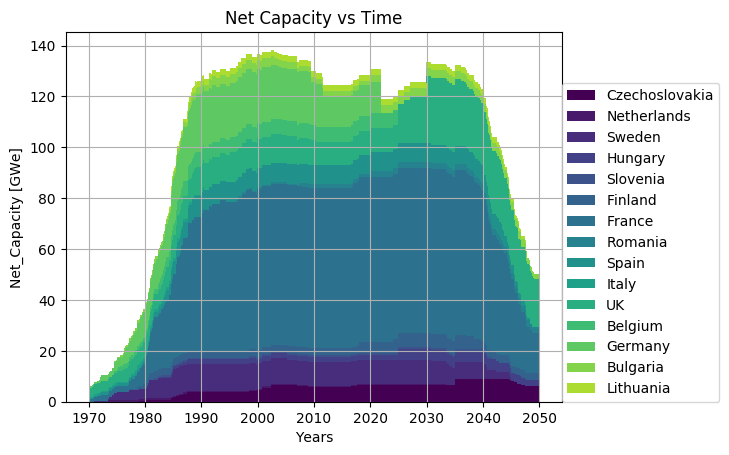
\includegraphics[width=.8\linewidth,height=.8\textheight,keepaspectratio]{./images/eu_future/power_plot.png}
		\end{center}
		\caption{Timeseries of installed nuclear capacity in \gls{EU}.}
		\label{fig:eu_pow}
	\end{figure}
	
\end{frame}

\begin{frame}
	\frametitle{Deployment Timeline for French Transition}
	110 \glspl{SFR} (66 GWe) are deployed by 2076.
	\begin{figure}[htbp!]
	\begin{minipage}[b]{.45\linewidth}
        \begin{center}
                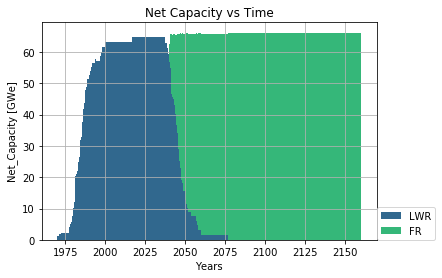
\includegraphics[width=\textwidth]{./images/french-transition/power_plot.png}
        \end{center}
        \caption{French Transition into an SFR Fleet}
        \label{fig:sfr_num}
	\end{minipage}
	\hspace{.5cm}
	\begin{minipage}[b]{.45\linewidth}
		\centering
		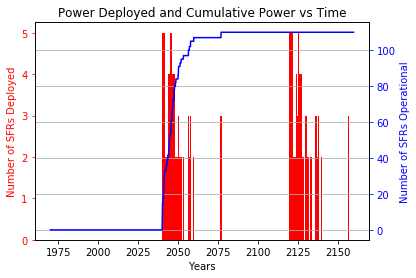
\includegraphics[width=\textwidth]{./images/french-transition/sfr_deploy.png}
		\caption{Deployment of French \glspl{SFR} and total installed capacity}
		\label{fig:dep}
	\end{minipage}
\end{figure}
\end{frame}
